% Lecture Template for ME3050 - Dynamic Modeling and Controls - Tennessee Technological University
% Spring 2024 - condensing and streamlining lectures by combining topics into a single PDF under the module name
% this will simplify file and link management as well as make lectures easier to use in class
% - added image/ to clean directory and reduce redundancy, specific to module for now  

% Module Name: - Laplace Transforms
% Topic 1 - The Laplace Transform
% Topic 2 - Laplace Transforms Method
% Topic 3 - Partial Fraction Decomposition

\documentclass[fleqn]{beamer} % for presentation (has nav buttons at bottom)

\usepackage{../dmc_lectures} % .sty in parent folder

\author{ME3050 - Dynamics Modeling and Controls}

\newcommand{\MNUM}{2\hspace{2mm}} % module number 
\newcommand{\moduletitle}{The Laplace Transform}

\newcommand{\sectionItitle}{The Laplace Transform}
\newcommand{\sectionIItitle}{Laplace Transforms Method}
\newcommand{\sectionIIItitle}{Partial Fraction Decomposition}

\newcommand{\sectionIsubsectionItitle}{An Integral Transform}
\newcommand{\sectionIsubsectionIItitle}{Laplace Transform of A Derivative}
\newcommand{\sectionIsubsectionIIItitle}{Properties of an Integral}
\newcommand{\sectionIsubsectionIVtitle}{Table of Transform Pairs}

\newcommand{\sectionIIsubsectionItitle}{Step 1 - Apply Laplace Transform}
\newcommand{\sectionIIsubsectionIItitle}{Step 2 - Solve for $X(s)$}
\newcommand{\sectionIIsubsectionIIItitle}{Step 3 - Rearrange to Find Invertable Form}
\newcommand{\sectionIIsubsectionIVtitle}{Step 4 - Invert for Final Answer}

\newcommand{\sectionIIIsubsectionItitle}{General Polynomial Form}
\newcommand{\sectionIIIsubsectionIItitle}{Case 1 - Distinct Roots}
\newcommand{\sectionIIIsubsectionIIItitle}{Case 2 - Repeated Roots}
\newcommand{\sectionIIIsubsectionIVtitle}{Special Case - Complex Roots}


% custom box
\newsavebox{\mybox}

\title{Lecture Module - \moduletitle}

\date{Mechanical Engineering\vspc Tennessee Technological University}

\begin{document}

	\lstset{language=MATLAB,basicstyle=\ttfamily\small,showstringspaces=false}

	\frame{\titlepage \center\begin{framed}\Large \textbf{Module \MNUM - \moduletitle}\end{framed} \vspace{5mm}}

	% Module Outline
	\begin{frame} 
		\large \textbf{Module \MNUM - \moduletitle} \vspace{3mm}\\

		\begin{itemize}
			\item Topic 1 - \hyperlink{sectionI}{\sectionItitle} \vspc % section I
			\item Topic 2 - \hyperlink{sectionII}{\sectionIItitle} \vspc % section II
			\item Topic 3 - \hyperlink{sectionIII}{\sectionIIItitle} \vspc % section III
		\end{itemize}

	\end{frame}

	% section I
	\section{\sectionItitle}\label{sectionI}

		% section I Outline
		\begin{frame} 
			\large \textbf{Topic 1 - \sectionItitle} \vspace{3mm}\\

			\begin{itemize}
				\item \hyperlink{sectionIsubsectionI}{\sectionIsubsectionItitle} \vspc %  section I subsection I
				\item \hyperlink{sectionIsubsectionII}{\sectionIsubsectionIItitle} \vspc % section I subsection II
				\item \hyperlink{sectionIsubsectionIII}{\sectionIsubsectionIIItitle} \vspc % section I subsection III
				%\item \hyperlink{sectionIsubsectionIV}{\sectionIsubsectionIVtitle} \vspc % section I subsection IV
			\end{itemize}
		\end{frame}
		
		% section I subsection I 
		\subsection{\sectionIsubsectionItitle}\label{sectionIsubsectionI}

			\begin{frame}
				\frametitle{\sectionIsubsectionItitle}
				\bigskip

 				The Laplace Transform is an Integral Transform

				Given a function $x(t)$ in the time domain where $t\geq0$, \\ the Laplace Transform is defined as follows: \\

				\[ X(s)=\Lagr{\{x(t)\}}=\displaystyle\int_0^{\infty} x(t)e^{-st}dt \]

				And its inverse is similarly defined as: \\

				\[ \Lagr^{-1}{\{X(s)\}}=x(t) \]

				The Laplace Domain variable $s$ is a complex number: \[ s=\sigma+j\omega \]
	
				\btVFill
			\end{frame}

			\begin{frame}
				\frametitle{\sectionIsubsectionItitle}
				\bigskip

	
 
  
				\btVFill
			\end{frame}

			\begin{frame}
				\frametitle{\sectionIsubsectionItitle}
				\bigskip


				\btVFill
			\end{frame}

		



		% section I subsection II
		\subsection{\sectionIsubsectionIItitle}\label{sectionIsubsectionII}

			\begin{frame}
				\frametitle{\sectionIsubsectionIItitle}
				\bigskip

					It is useful to find the laplace transform of the derivative of a function: 
					\[ \Lagr{\{\frac{d}{dt}(x(t))\} }=\Lagr{\{\dot{x}(t)\}} =s\Lagr{\{x(t)\} }-x(t=0) \]
					\[ \hspace{52mm} =sX(s)-x(t=0) \]
					\[ \hspace{52mm}\Lagr{\{ \dot{x} \left(t\right) \}} =sX(s)-x_0 \]

					\[ \Lagr{\{\frac{d^2}{dt^2}(x(t))\} }=\Lagr{\{\ddot{x}(t)\}} = s^2\Lagr{\{x(t)\} }-sx(t=0)-\dot{x}(t=0) \]
					\[ \hspace{52mm} = s^2X(s)-sx(t=0)-\dot{x}(t=0) \]
					\[ \hspace{52mm} \Lagr{\{ \ddot{x} \left(t\right) \}}= s^2X(s)-sx_0-\dot{x}_0  \]

				\btVFill
			\end{frame}

				%\btVFill
			\begin{frame}
				\frametitle{\sectionIsubsectionIItitle}
				\bigskip
				

				  
		
				\btVFill
			\end{frame}

		% section I subsection III
		\subsection{\sectionIsubsectionIIItitle}\label{sectionIsubsectionIII}
			\begin{frame} 
				\frametitle{\sectionIsubsectionIIItitle}
				\bigskip

				Also, remember that the transform inherits the properties of an integral.

				\[ \int\left[ x(t)+y(t) \right]dt =\int x(t)dt + \int y(t)dt \]
				\[ \int Kx(t)dt = K\int x(t)dt \hspcc (K \hspc is \hspc constant)\]

				Therefore these properties can be used with the Laplace transform.	
								
				\btVFill
			\end{frame}	


		% section I subsection IV
		\subsection{\sectionIsubsectionIVtitle}\label{sectionIsubsectionIV}

			\begin{frame}
				\frametitle{\sectionIsubsectionIVtitle}
				\bigskip

				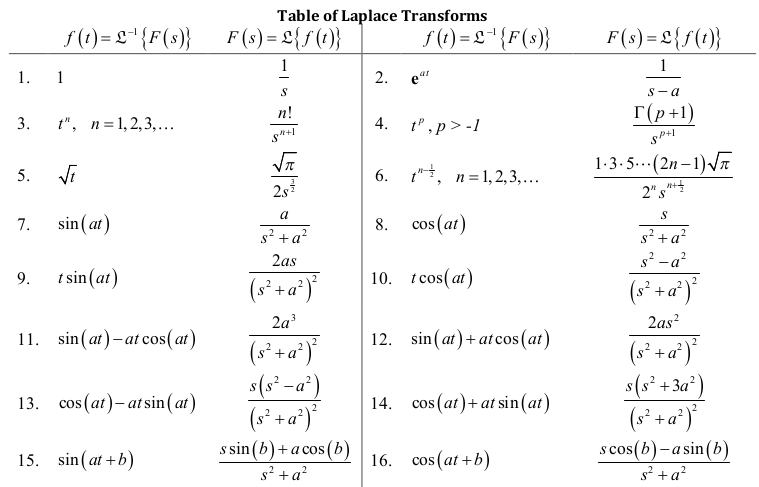
\includegraphics[scale=.35]{images/laplace_table_part1.png}
					
				\btVFill
			\end{frame}	

			\begin{frame}
				\frametitle{\sectionIsubsectionIVtitle}
				\bigskip

				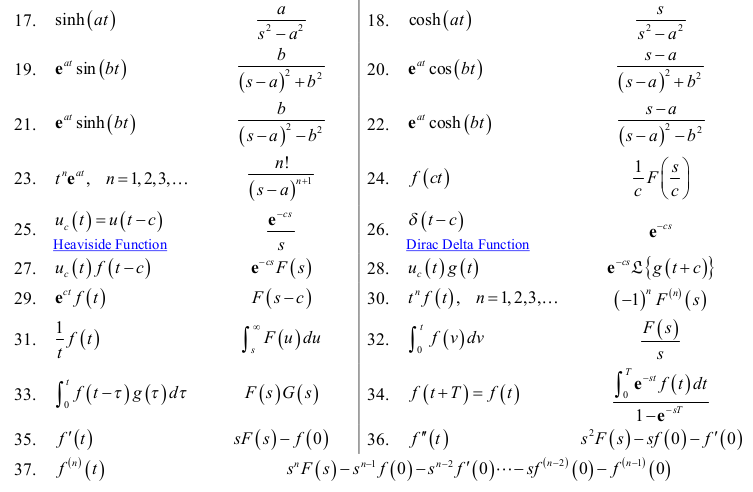
\includegraphics[scale=.35]{images/laplace_table_part2.png}

				\btVFill
			\end{frame}	

	
	% Section II
	\section{\sectionIItitle}\label{sectionII}

		% section II Outline
		\begin{frame}
			\large \textbf{Topic 2 - \sectionIItitle} \vspace{3mm}\\

			\begin{itemize}
				\item \hyperlink{sectionIIsubsectionI}{\sectionIIsubsectionItitle} \vspc %  section II subsection I
				\item \hyperlink{sectionIIsubsectionII}{\sectionIIsubsectionIItitle} \vspc % section II subsection II
				\item \hyperlink{sectionIIsubsectionIII}{\sectionIIsubsectionIIItitle} \vspc % section II subsection III
				%\item \hyperlink{sectionIIsubsectionIV}{\sectionIIsubsectionIVtitle} \vspc % section II subsection IV
			\end{itemize}

		\end{frame}

		% section II subsection I
		\subsection{\sectionIIsubsectionItitle}\label{sectionIIsubsectionI}

			\begin{frame}[label=sectionIIsubsectionI]
				\frametitle{\sectionIIsubsectionItitle}
				\bigskip

				Example:

				Solve the first order differential equation using the Laplace Transforms Method with the initial condition given. 
				\[4\dot{x}=sin\left(t\right) \hspccc with \hspccc x\left(t=0\right)=x_0 \] 
				Apply the Laplace Transform to both sides of the differential equation. 

				\[ 4\left(sX\left(s \right)-x_0 \right)=\frac{1}{s^2+1} \]
				
				\btVFill
			\end{frame}


		% section II subsection II
		\subsection{\sectionIIsubsectionIItitle}\label{sectionIIsubsectionII}

			\begin{frame}

				\frametitle{\sectionIIsubsectionIItitle}
				\bigskip

				This step can seem open ended...
				\[X(s)=\frac{1}{4s\left(s^2+1\right)}+\frac{x_0}{s} \] 
	
				\btVFill 
			\end{frame}

			\begin{frame}

				\frametitle{\sectionIIsubsectionIItitle}
				\bigskip



				\btVFill 
			\end{frame}




		% section II subsection III
		\subsection{\sectionIIsubsectionIIItitle}\label{sectionIIsubsectionIII}

			\begin{frame}
				\frametitle{\sectionIIsubsectionIIItitle}
				\bigskip

				Write $X\left(s\right)$ in a form that can be inverted using the table of Laplace transform pairs. This typically involves partial fraction decomposition. 
				\[\frac{1}{4s\left(s^2+1 \right)}=\frac{1/4}{s\left(s^2+1\right)} =\frac{a}{s}+\frac{bs+c}{s^2+1} \] 

				Mulitply through by the denominator $4s\left(s^2+1\right)$:
				\[ 1=4as\left(s^2+1\right)+4s\left(bs+c\right)=4\left(a+b \right)s^2 + 4cs +4a \]

				Solve for the coefficients by {\it equating coefficients}.

				\[ \left( a+b\right)=0 \hspcc c=0 \hspcc a=\frac{1}{4} \implies a=\frac{1}{4} \hspcc b=-\frac{1}{4} \hspcc c=0 \]	
			
				\btVFill 
			\end{frame}	


			\begin{frame}
				\frametitle{\sectionIIsubsectionIItitle}
				\bigskip

				
				
				\btVFill 
			\end{frame}	


			\begin{frame}
				\frametitle{\sectionIIsubsectionIIItitle}
				\bigskip

				
				\btVFill 
			\end{frame}

			
		% section II subsection IV
		\subsection{\sectionIIsubsectionIVtitle}\label{sectionIIsubsectionIV}

			\begin{frame}
				\frametitle{\sectionIIsubsectionIVtitle}
				\bigskip
				Substitute the coefficients into $X(s)$,

				\[ X(s) =\frac{x_0}{s}+\frac{1}{4s}-\frac{s}{4\left(s^2+1\right)} \]

				and use the inverse transform to solve for $x(t)$. Use the Table.

				\[ \Lagr^{-1} \left( X\left( s\right)\right)=x(t)= \]
				\[ = x_0+\frac{1}{4}-\frac{1}{4}cos\left(t\right)=x_0+\frac{1}{4}\left(1-cos\left(t\right) \right) \]

				This method works for complex problems but it can get messy...	
			
				\btVFill 
			\end{frame}	

			\begin{frame}
				\frametitle{\sectionIIsubsectionIVtitle}
				\bigskip
				
				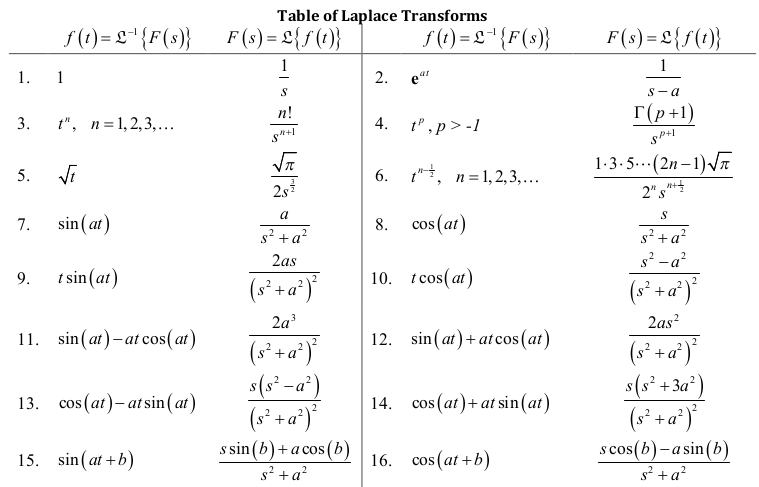
\includegraphics[scale=.35]{images/laplace_table_part1.png}

				\btVFill 
			\end{frame}	

			\begin{frame}
				\frametitle{\sectionIIsubsectionIVtitle}
				\bigskip
				
				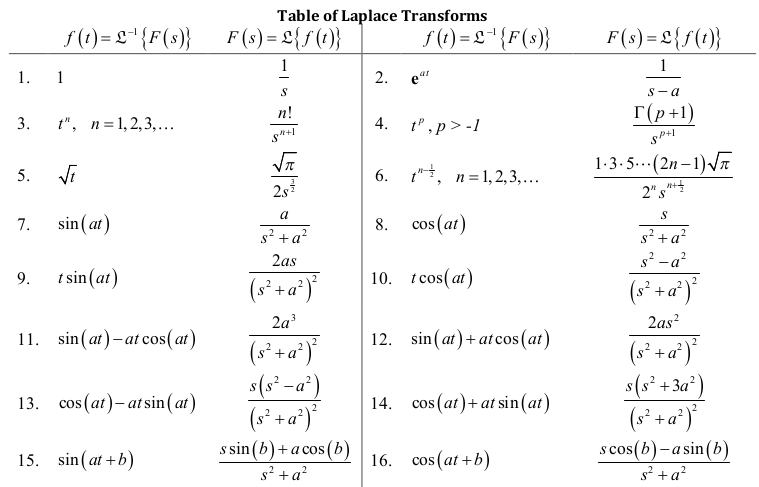
\includegraphics[scale=.35]{images/laplace_table_part1.png}

				\btVFill 
			\end{frame}	


		
	% Section III
	\section{\sectionIIItitle}\label{sectionIII}

		% section III Outline
		\begin{frame}
			\large \textbf{Topic 3 - \sectionIIItitle} \vspace{3mm}\\

			\begin{itemize}
				\item \hyperlink{sectionIIIsubsectionI}{\sectionIIIsubsectionItitle} \vspc %  section III subsection I
				\item \hyperlink{sectionIIIsubsectionII}{\sectionIIIsubsectionIItitle} \vspc % section III subsection II
				\item \hyperlink{sectionIIIsubsectionIII}{\sectionIIIsubsectionIIItitle} \vspc % section III subsection III
				\item \hyperlink{sectionIIIsubsectionIV}{\sectionIIIsubsectionIVtitle} \vspc % section III subsection IV
				%\item \hyperlink{sectionIIIsubsectionV}{\sectionIIIsubsectionVtitle} \vspc % section III subsection V
			\end{itemize}

		\end{frame}

		% section III subsection I
		\subsection{\sectionIIIsubsectionItitle}\label{sectionIIIsubsectionI}

			\begin{frame}
				\frametitle{\sectionIIIsubsectionItitle}
				\bigskip

				\textbf{The Laplace Transform is an Integral Transform: } \\

				Given a function $x(t)$ in the time domain where $t\geq0$, \\ the Laplace Transform is defined as follows: \\

				\[ X(s)=\Lagr{\{x(t)\}}=\displaystyle\int_0^{\infty} x(t)e^{-st}dt \]

				Partial Fraction Expansion leads to a general form:  \\

				\[ X(s)=\frac{N(s)}{D(s)}=\frac{b_ms^m+b_{m-1}+...+b_1s+b_0}{s^n+a_{n-1}s^{n-1}+...+a_1s+a_0 \hspace{5mm} n\geq m}\] 

				\btVFill
			\end{frame}

			\begin{frame}
				\frametitle{\sectionIIIsubsectionItitle}
				\bigskip
				

				\btVFill
			\end{frame}

		% section III subsection II
		\subsection{\sectionIIIsubsectionIItitle}\label{sectionIIIsubsectionII}	

			\begin{frame}
				\frametitle{\sectionIIIsubsectionIItitle}
				\bigskip

				\textbf{Case 1 - Distinct Roots: n roots are real and distinct} 

				The general form is factored:
				\[ X(s)=\frac{N(s)}{(s+r_1)(s+r_2)...(s+r_n)} \]

				The fraction will expand to: 
				\[ X(s)=\frac{C_1}{(s+r_1)}+\frac{C_2}{(s+r_2)}+...+\frac{C_n}{(s+r_n)} \]  
				
				Where:
				\[ \displaystyle C_i=\lim_{s\rightarrow-r_i}\{ X(s)(s+r_i) \} \]

				And this leads to a solution: 
				\[x(t)=C_1e^{-r_1t}+C_2e^{-r_2t}+...+C_ne^{-r_nt} \]
	
				\btVFill
			\end{frame}

		% section III subsection III
		\subsection{\sectionIIIsubsectionIIItitle}\label{sectionIIIsubsectionIII}

			\begin{frame}
				\frametitle{\sectionIIIsubsectionIIItitle}
				\bigskip

				\textbf{Case 2 - Repeated Roots: p number of roots have the same value $(s =-r)$ and remaining roots are distinct and real distinct} 
	
				\[X(s)=\frac{N(s)}{(s+r_1)^p(s+r_{p+1})(s+r_{p+2})...(s+r_n)} \]

				The fraction will expand to: \\

				\[X(s)=\frac{C_1}{(s+r_1)^p}+\frac{C_2}{(s+r_1)^{p-1}}+...\] 
				\[ +\frac{C_p}{(s+r_1)}+\frac{C_{p+1}}{(s+r_{p+1})}+...+\frac{C_n}{(s+r_n)} \]
			
				\btVFill
			\end{frame}

			\begin{frame}
				\frametitle{\sectionIIIsubsectionIIItitle}
				\bigskip

				Coefficients for the repeated root are:\\

				\[\displaystyle C_1=\lim_{s\rightarrow-r_i}\{X(s)(s+r_i)^p\} \]
				\[\displaystyle C_2=\lim_{s\rightarrow-r_i}\{\frac{d}{ds}X(s)(s+r_i)^p\} \]
				
				\[ \displaystyle C_i=\lim_{s\rightarrow-r_i}\{\frac{1}{(i-1)!}\frac{d^{(i-1)}}{ds^{(i-1)}}X(s)(s+r_i)^p\} \]

				Coefficients for the distinct roots are the same as in Case 1:\\

				And this leads to a solution: \\

				\[ x(t)=C_1\frac{t^{p-1}}{(p-1)!}e^{-r_1t}+C_2\frac{t^{p-2}}{(p-2)!}e^{-r_1t}+...\]
				\[ ...+C_{p}e^{-r_1t}+C_{p+1}e^{-r_{p+1}t}...+C_ne^{-r_nt} \]
			
				\btVFill
			\end{frame}

		% section III subsection IV
		\subsection{\sectionIIIsubsectionIVtitle}\label{sectionIIIsubsectionIV}	

			\begin{frame}
				\frametitle{\sectionIIIsubsectionIVtitle}
				\bigskip

				\textbf{Special Case - Complex Roots: the roots are distinct $\implies$ Case 1} 

				Example:

				\[ X(s)=\left[ \frac{3s+7}{\left(4s^2+24s+136\right)} \right]=\left[ \frac{3s+7}{4\left(s^2+6s+34\right)} \right] \]

				The solution can be found by forming two perfect squares in the denominator.

				\[ X(s)=\frac{1}{4} \left[ \frac{3s+7}{\left(s+3\right)^2+5^2}\right] \]

				\btVFill 
			\end{frame}

			\begin{frame}
				\frametitle{\sectionIIIsubsectionIVtitle}
				\bigskip

				Now this can be expanded into the following terms which can be found in the table!

				\[ X(s)=\frac{1}{4}  \left[ C_1 \frac{5}{\left(s+3\right)^2+5^2} +C_2 \frac{s+3}{\left(s+3\right)^2+5^2}\right] \]

				Multiply by the denominator and solve for $C_1$ and $C_2$.

				\[ 3s+7 = 5C_1 +C_2\left( s+3\right) = 5C_1 +c_2s+3C_2 \implies C_2=3, C_1 = -\frac{2}{5} \]

		 		\btVFill 
			\end{frame}
			
			\begin{frame}
				\frametitle{\sectionIIIsubsectionIVtitle}
				\bigskip
				
				Finally substitute and invert using the table. 

				\[ X(s)=\frac{1}{4}  \left[-\frac{2}{5}\frac{5}{\left(s+3\right)^2+s^2} +3 \frac{s+3}{\left(s+3\right)^2+s^2}\right] \] 

				Write the final answer in the time domain.
				\[ x(t) =-\frac{1}{10}e^{-3t}sin\left(5t\right)+\frac{3}{4}e^{-3t}cos\left(5t\right) \]
					
				\btVFill 
			\end{frame}

			\begin{frame}
				\frametitle{\sectionIIIsubsectionIVtitle}
				\bigskip
			
				
				\btVFill 
			\end{frame}


\end{document}





